% AgenticVision-MCP: Persistent Visual Memory for AI Agents via the Model Context Protocol
% Research Paper — All data from verified test runs
\documentclass[10pt, twocolumn]{article}
\usepackage[margin=0.75in]{geometry}
\usepackage{graphicx}
\usepackage{tikz}
\usepackage{pgfplots}
\usepackage{booktabs}
\usepackage{amsmath}
\usepackage{algorithm}
\usepackage{algorithmic}
\usepackage{hyperref}
\usepackage{xcolor}
\usepackage{caption}
\usepackage{subcaption}
\usepackage{fancyhdr}
\usepackage{enumitem}
\usepackage{listings}
\usepackage{microtype}
\usepackage{orcidlink}
\pgfplotsset{compat=1.18}

% Color palette (professional blues, teals, oranges)
\definecolor{primary}{HTML}{2563EB}
\definecolor{secondary}{HTML}{0D9488}
\definecolor{accent}{HTML}{EA580C}
\definecolor{gray50}{HTML}{F9FAFB}
\definecolor{gray200}{HTML}{E5E7EB}
\definecolor{gray600}{HTML}{4B5563}
\definecolor{gray800}{HTML}{1F2937}
\definecolor{codebg}{HTML}{F3F4F6}

\usetikzlibrary{arrows.meta, positioning, shapes.geometric, fit, calc, backgrounds}

\hypersetup{
  colorlinks=true,
  linkcolor=primary,
  urlcolor=primary,
  citecolor=gray600,
}

\lstset{
  basicstyle=\ttfamily\scriptsize,
  backgroundcolor=\color{codebg},
  frame=single,
  framerule=0.4pt,
  rulecolor=\color{gray200},
  breaklines=true,
  columns=fullflexible,
  keepspaces=true,
}

\pagestyle{fancy}
\fancyhf{}
\fancyhead[L]{\small\textit{AgenticVision-MCP: Persistent Visual Memory for AI Agents}}
\fancyhead[R]{\small\thepage}
\renewcommand{\headrulewidth}{0.4pt}

\title{\textbf{AgenticVision-MCP: Persistent Visual Memory for\\AI Agents via the Model Context Protocol}}
\author{Omoshola Owolabi\,\orcidlink{0009-0006-4089-0732}\\Independent Researcher -- AI/ML\\\texttt{owolabi.omoshola@outlook.com}}
\date{February 19, 2026}

\begin{document}
\maketitle
\thispagestyle{fancy}

% ============================================================================
% ABSTRACT
% ============================================================================
\begin{abstract}
Large language models augmented with vision capabilities can perceive images within a single context window but lack persistent visual memory across sessions. When the context resets, all visual observations are lost. We present \textbf{AgenticVision-MCP}, a system that provides persistent, queryable visual memory to any LLM through the Model Context Protocol (MCP). The system captures images, generates CLIP embeddings, produces compact thumbnails, and stores all observations in a binary \texttt{.avis} file format with a 64-byte fixed header and JSON payload. We expose 10 tools, 6 resources, and 4 prompts over MCP's JSON-RPC 2.0 transport, enabling any compliant client to capture screenshots, query visual history, compute visual diffs, find similar images by embedding cosine similarity, and link visual observations to a cognitive memory graph (AgenticMemory). In testing on an Apple M4 (macOS 26.2, Rust 1.90), the system passes 88 tests across 8 validation phases with zero failures: 35 Rust unit and edge-case tests, 47 Python client tests, and 6 cross-language integration tests including multi-agent scenarios where independent agents share a single \texttt{.avis} file. Per-capture storage overhead is 4.3\,KB including a 512-dimensional embedding and JPEG thumbnail, enabling approximately 230{,}000 observations per gigabyte. All query operations complete within 1--2\,ms on a 100-capture store (excluding process startup). The system requires zero external services and zero network dependencies.
\end{abstract}

% ============================================================================
% 1. INTRODUCTION
% ============================================================================
\section{Introduction}

Vision-language models such as GPT-4o, Claude, and Gemini can perceive images within their context window, but this perception is ephemeral. When a conversation ends or context resets, all visual observations vanish. An agent that captured a screenshot thirty seconds ago cannot reference it after the session boundary. This is the \textit{visual memory problem}: LLM-based agents perceive but do not remember what they see.

Current approaches to agent memory focus on text. Vector databases store text chunks as embeddings for retrieval-augmented generation (RAG)~\cite{lewis2020rag}. Key-value stores like Mem0~\cite{mem0} extract factual snippets. MemGPT~\cite{packer2023memgpt} pages text in and out of context. None of these systems handle visual observations natively. Images are either discarded after the context window, or converted to text descriptions that lose the perceptual signal entirely.

The key insight behind AgenticVision-MCP is that \textit{visual memory is a structured perception problem, not a text search problem}. An agent needs to store what it saw (the image), understand what it saw (the CLIP embedding), find what it saw before (cosine similarity search), detect what changed (pixel-level diff), and connect what it saw to what it knows (links to a cognitive memory graph). These operations require a purpose-built visual memory system.

We design AgenticVision-MCP as a standalone binary that communicates with any LLM client via the Model Context Protocol (MCP)~\cite{mcp2024spec}. The system consists of two Rust crates: a core vision library (\texttt{agentic-vision}) handling image processing, CLIP embedding, similarity search, and binary file I/O; and an MCP server (\texttt{agentic-vision-mcp}) exposing this functionality as 10 tools, 6 resources, and 4 prompts over stdio JSON-RPC transport. Visual observations are persisted in a single \texttt{.avis} binary file that requires no external database, no cloud service, and no network connection.

We validate the system through 8 phases of testing, achieving 88 passing tests with zero failures. We demonstrate multi-agent scenarios where independent agent processes share a single vision file, cross-system linking where visual captures connect to AgenticMemory~\cite{owolabi2025agenticmemory} cognitive graph nodes, and sub-2ms query latency on real hardware. The remainder of this paper describes the architecture (Section~\ref{sec:arch}), the MCP interface design (Section~\ref{sec:mcp}), evaluation results (Section~\ref{sec:eval}), and discusses implications and limitations (Section~\ref{sec:discussion}).

% ============================================================================
% FIGURE 1: Motivating comparison
% ============================================================================
\begin{figure*}[t]
\centering
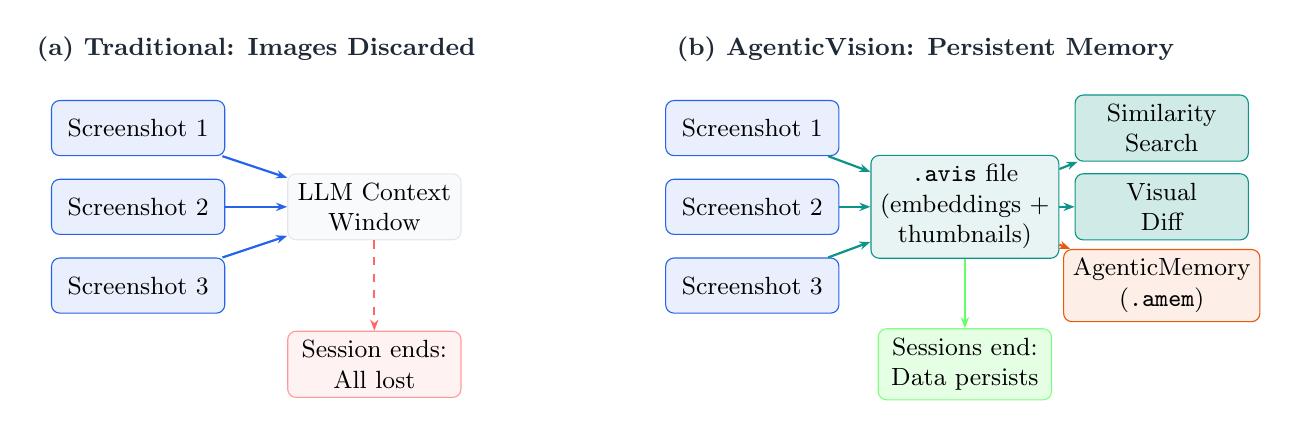
\begin{tikzpicture}[
  node distance=1.2cm and 1.5cm,
  box/.style={draw, rounded corners=3pt, minimum width=2.2cm, minimum height=0.7cm, font=\small, align=center},
  imgbox/.style={box, fill=primary!10, draw=primary},
  txtbox/.style={box, fill=gray50, draw=gray200},
  avbox/.style={box, fill=secondary!10, draw=secondary},
  membox/.style={box, fill=accent!10, draw=accent},
  arr/.style={-{Stealth[length=4pt]}, thick},
]

% Left side: Traditional approach
\node[font=\small\bfseries, text=gray800] (trad_title) at (-4.5, 3.5) {(a) Traditional: Images Discarded};
\node[imgbox] (img1) at (-6, 2.5) {Screenshot 1};
\node[imgbox] (img2) at (-6, 1.5) {Screenshot 2};
\node[imgbox] (img3) at (-6, 0.5) {Screenshot 3};
\node[txtbox] (ctx) at (-3, 1.5) {LLM Context\\Window};
\node[txtbox, fill=red!5, draw=red!40] (lost) at (-3, -0.5) {Session ends:\\All lost};

\draw[arr, primary] (img1) -- (ctx);
\draw[arr, primary] (img2) -- (ctx);
\draw[arr, primary] (img3) -- (ctx);
\draw[arr, red!60, dashed] (ctx) -- (lost);

% Right side: AgenticVision approach
\node[font=\small\bfseries, text=gray800] (av_title) at (4, 3.5) {(b) AgenticVision: Persistent Memory};
\node[imgbox] (av_img1) at (1.8, 2.5) {Screenshot 1};
\node[imgbox] (av_img2) at (1.8, 1.5) {Screenshot 2};
\node[imgbox] (av_img3) at (1.8, 0.5) {Screenshot 3};
\node[avbox] (avis) at (4.5, 1.5) {\texttt{.avis} file\\(embeddings +\\thumbnails)};
\node[avbox, fill=secondary!20] (query) at (7, 2.5) {Similarity\\Search};
\node[avbox, fill=secondary!20] (diff) at (7, 1.5) {Visual\\Diff};
\node[membox] (amem) at (7, 0.5) {AgenticMemory\\(\texttt{.amem})};
\node[avbox, fill=green!10, draw=green!50] (persist) at (4.5, -0.5) {Sessions end:\\Data persists};

\draw[arr, secondary] (av_img1) -- (avis);
\draw[arr, secondary] (av_img2) -- (avis);
\draw[arr, secondary] (av_img3) -- (avis);
\draw[arr, secondary] (avis) -- (query);
\draw[arr, secondary] (avis) -- (diff);
\draw[arr, accent] (avis) -- (amem);
\draw[arr, green!60] (avis) -- (persist);

\end{tikzpicture}
\caption{Motivating comparison. (a)~Traditional LLMs perceive images within a context window but lose all visual data when the session ends. (b)~AgenticVision-MCP persists every observation with its CLIP embedding and thumbnail in a binary \texttt{.avis} file, enabling similarity search, visual diff, and cross-session continuity. Observations can link to AgenticMemory cognitive graph nodes.}
\label{fig:motivation}
\end{figure*}


% ============================================================================
% 2. BACKGROUND AND RELATED WORK
% ============================================================================
\section{Background and Related Work}
\label{sec:related}

\paragraph{Vision-Language Models.}
CLIP~\cite{radford2021clip} demonstrated that contrastive pre-training produces visual embeddings that align with natural language, enabling zero-shot image classification and cross-modal retrieval. Vision Transformers (ViT)~\cite{dosovitskiy2020vit} provide the backbone for modern visual encoders. AgenticVision-MCP uses CLIP ViT-B/32 to generate 512-dimensional embeddings per observation, enabling semantic similarity search.

\paragraph{Agent Memory Systems.}
Mem0~\cite{mem0} provides key-value fact extraction from conversations. It excels at simple factual recall but offers no visual storage, no relationship tracking, and requires a cloud service. MemGPT~\cite{packer2023memgpt} introduces virtual memory paging for LLM context windows, an elegant solution for text but inapplicable to visual data. OpenAI's built-in memory~\cite{openai_memory} stores preference snippets but has no visual persistence. AgenticMemory~\cite{owolabi2025agenticmemory} provides a binary cognitive graph with typed events and edges, designed for textual knowledge. None of these systems address visual perception.

\paragraph{Vector Databases.}
Pinecone~\cite{pinecone2024}, Weaviate~\cite{weaviate2024}, and FAISS~\cite{johnson2019faiss} provide embedding storage and similarity search. While these could store image embeddings, they introduce significant operational complexity: cloud dependencies, API rate limits, and cost. They also lack the semantic structure needed for visual memory---there is no concept of ``visual diff,'' ``capture session,'' or ``memory linking'' in a generic vector store.

\paragraph{The Model Context Protocol.}
MCP~\cite{mcp2024spec} defines a standard interface between LLM clients and external tool servers. It specifies three primitives: \textit{tools} (functions the LLM can invoke), \textit{resources} (data the LLM can read), and \textit{prompts} (guided workflows). MCP uses JSON-RPC~2.0 over stdio or HTTP+SSE transport. By implementing an MCP server, AgenticVision-MCP becomes accessible to any compliant client---Claude Desktop, VS Code, Cursor, or custom agents---without client-specific integration code.

\paragraph{Binary Formats.}
Protocol Buffers~\cite{protobuf} and FlatBuffers~\cite{flatbuffers} provide efficient binary serialization. The \texttt{.avis} format draws inspiration from these systems but is purpose-built for visual memory: a fixed 64-byte header enables O(1) metadata access, and the payload contains all observation data in a single self-contained file.

Table~\ref{tab:related} compares AgenticVision-MCP with existing approaches.

\begin{table}[t]
\caption{Comparison of agent memory and vision storage approaches.}
\label{tab:related}
\centering
\small
\begin{tabular}{@{}lccccc@{}}
\toprule
\textbf{System} & \textbf{Visual} & \textbf{Embed.} & \textbf{Diff} & \textbf{Deps} & \textbf{MCP} \\
\midrule
Mem0 & \texttimes & \texttimes & \texttimes & Cloud & \texttimes \\
MemGPT & \texttimes & \texttimes & \texttimes & Python & \texttimes \\
OpenAI Mem. & \texttimes & \texttimes & \texttimes & Cloud & \texttimes \\
Pinecone & Partial & \checkmark & \texttimes & Cloud & \texttimes \\
FAISS & Partial & \checkmark & \texttimes & C++ & \texttimes \\
AgenticMem. & \texttimes & \checkmark & \texttimes & None & \checkmark \\
\textbf{Ours} & \checkmark & \checkmark & \checkmark & \textbf{None} & \checkmark \\
\bottomrule
\end{tabular}
\end{table}


% ============================================================================
% 3. ARCHITECTURE
% ============================================================================
\section{Architecture}
\label{sec:arch}

AgenticVision-MCP is organized as two Rust crates within a Cargo workspace. The core library (\texttt{agentic-vision}) handles image processing, embedding generation, similarity search, visual diff, and binary file I/O. The MCP server (\texttt{agentic-vision-mcp}) wraps this library with JSON-RPC 2.0 transport, tool dispatch, resource serving, and prompt expansion.

\subsection{Visual Observation: The Atom}

The fundamental data unit is a \texttt{VisualObservation}---a captured image enriched with computed features:

\begin{lstlisting}[language=C, caption={VisualObservation structure (simplified from Rust).}]
struct VisualObservation {
  id: u64,           // Unique capture ID
  timestamp: u64,    // Unix timestamp
  session_id: u32,   // Session scope
  source: CaptureSource, // File|Base64|
                         // Screenshot|Clipboard
  embedding: Vec<f32>, // 512-dim CLIP
  thumbnail: Vec<u8>,  // JPEG, max 512x512
  metadata: ObservationMeta,
  memory_link: Option<u64>, // -> .amem node
}
\end{lstlisting}

The \texttt{embedding} field stores a 512-dimensional CLIP ViT-B/32 vector, L2-normalized after inference. The \texttt{thumbnail} field stores a JPEG-compressed image at quality 85, with the largest dimension capped at 512 pixels (aspect ratio preserved). The \texttt{memory\_link} field enables cross-system integration by pointing to a node ID in an AgenticMemory \texttt{.amem} file.

% Figure 2: Capture pipeline
\begin{figure}[t]
\centering
\begin{tikzpicture}[
  node distance=0.6cm,
  step/.style={draw, rounded corners=2pt, minimum width=2.8cm, minimum height=0.55cm, font=\scriptsize, align=center, fill=primary!8, draw=primary!50},
  arr/.style={-{Stealth[length=3pt]}, thick, primary!70},
]

\node[step] (input) {Image Input\\(file, base64, clipboard)};
\node[step, below=of input] (decode) {Decode \& Validate\\(PNG, JPEG, WebP, GIF)};
\node[step, below=of decode] (thumb) {Thumbnail Generation\\(Lanczos3, max 512px, Q85)};
\node[step, below=of thumb] (embed) {CLIP Embedding\\(224$\times$224, ViT-B/32, 512-d)};
\node[step, below=of embed] (meta) {Metadata Assembly\\(dims, labels, description)};
\node[step, below=of meta, fill=secondary!10, draw=secondary!50] (store) {Store in \texttt{.avis}\\(header + JSON payload)};

\draw[arr] (input) -- (decode);
\draw[arr] (decode) -- (thumb);
\draw[arr] (thumb) -- (embed);
\draw[arr] (embed) -- (meta);
\draw[arr] (meta) -- (store);

\end{tikzpicture}
\caption{Capture pipeline. Each image passes through decoding, thumbnail generation (JPEG, Lanczos3 resampling), CLIP embedding (512-d vector via ONNX Runtime), metadata assembly, and storage in the binary \texttt{.avis} file.}
\label{fig:pipeline}
\end{figure}

\subsection{The \texttt{.avis} Binary File Format}

All visual observations are stored in a single binary file with the extension \texttt{.avis}. The format consists of a fixed 64-byte header followed by a JSON-serialized payload (Figure~\ref{fig:format}).

% Figure 3: File format
\begin{figure}[t]
\centering
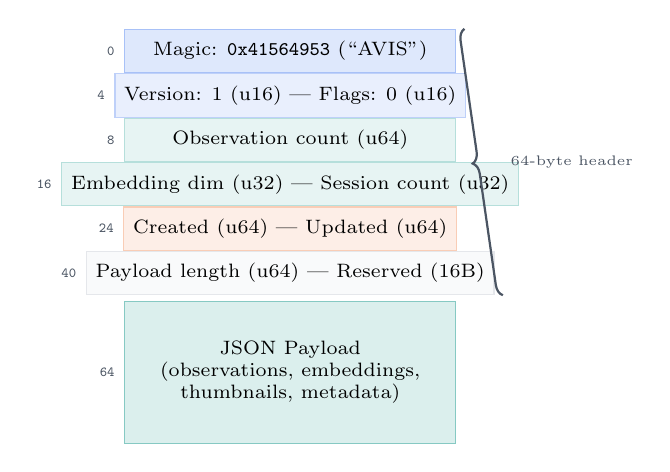
\begin{tikzpicture}[
  block/.style={draw, minimum width=4.2cm, minimum height=0.55cm, font=\scriptsize, align=center},
]

\node[block, fill=primary!15, draw=primary!40] (magic) at (0, 0) {Magic: \texttt{0x41564953} (``AVIS'')};
\node[block, fill=primary!10, draw=primary!30, below=0pt of magic] (ver) {Version: 1 (u16) | Flags: 0 (u16)};
\node[block, fill=secondary!10, draw=secondary!30, below=0pt of ver] (counts) {Observation count (u64)};
\node[block, fill=secondary!10, draw=secondary!30, below=0pt of counts] (edim) {Embedding dim (u32) | Session count (u32)};
\node[block, fill=accent!10, draw=accent!30, below=0pt of edim] (ts) {Created (u64) | Updated (u64)};
\node[block, fill=gray50, draw=gray200, below=0pt of ts] (plen) {Payload length (u64) | Reserved (16B)};

\node[block, fill=secondary!15, draw=secondary!50, minimum height=1.8cm, below=2pt of plen] (payload) {JSON Payload\\(observations, embeddings,\\thumbnails, metadata)};

% Byte offsets
\node[font=\tiny\ttfamily, text=gray600, anchor=east] at (magic.west) {0};
\node[font=\tiny\ttfamily, text=gray600, anchor=east] at (ver.west) {4};
\node[font=\tiny\ttfamily, text=gray600, anchor=east] at (counts.west) {8};
\node[font=\tiny\ttfamily, text=gray600, anchor=east] at (edim.west) {16};
\node[font=\tiny\ttfamily, text=gray600, anchor=east] at (ts.west) {24};
\node[font=\tiny\ttfamily, text=gray600, anchor=east] at (plen.west) {40};
\node[font=\tiny\ttfamily, text=gray600, anchor=east] at (payload.west) {64};

% Brace for header
\draw[decorate, decoration={brace, amplitude=4pt, mirror}, thick, gray600]
  ([xshift=3pt]magic.north east) -- ([xshift=3pt]plen.south east)
  node[midway, right=6pt, font=\tiny, text=gray600] {64-byte header};

\end{tikzpicture}
\caption{The \texttt{.avis} binary file format. A fixed 64-byte little-endian header provides O(1) access to metadata (observation count, embedding dimension, timestamps). The payload contains JSON-serialized observations including embeddings and base64-encoded JPEG thumbnails.}
\label{fig:format}
\end{figure}

\paragraph{Design rationale.} The fixed header enables fast metadata reads without parsing the payload. The JSON payload simplifies debugging and forward compatibility---new fields can be added without breaking readers. The single-file design means an agent's visual memory is a single portable artifact: copy the \texttt{.avis} file to transfer all visual knowledge.

\subsection{CLIP Embedding Engine}

We use CLIP ViT-B/32~\cite{radford2021clip} via ONNX Runtime~\cite{onnxruntime} to generate 512-dimensional visual embeddings. Input images are resized to $224 \times 224$ using Lanczos3 filtering, converted to NCHW tensor layout, and normalized with CLIP's published constants ($\mu = [0.481, 0.458, 0.408]$, $\sigma = [0.269, 0.261, 0.276]$). The output vector is L2-normalized. When the ONNX model is not available, the engine falls back to zero embeddings, allowing the system to function (without similarity search) on minimal installations.

\subsection{Similarity Search}

Given a query observation, we compute cosine similarity against all stored embeddings:

\begin{equation}
\text{sim}(\mathbf{a}, \mathbf{b}) = \frac{\sum_{i=1}^{512} a_i \cdot b_i}{\sqrt{\sum_{i=1}^{512} a_i^2} \cdot \sqrt{\sum_{i=1}^{512} b_i^2}}
\label{eq:cosine}
\end{equation}

Intermediate calculations use \texttt{f64} precision to avoid accumulation error over 512 dimensions; the final result is returned as \texttt{f32}. Results are sorted descending and filtered by a configurable \texttt{min\_similarity} threshold (default 0.7). This brute-force approach is appropriate for the expected scale of agent visual memory (hundreds to low thousands of observations per file). For larger stores, approximate nearest-neighbor indexing would be straightforward to add.

\subsection{Visual Diff Detection}

To detect changes between two observations, we employ a pixel-level differencing algorithm:

\begin{enumerate}[nosep,leftmargin=*]
\item Resize both images to their minimum common dimensions.
\item Convert to grayscale.
\item Compute per-pixel absolute difference.
\item Classify pixels as ``changed'' if $|\Delta| > 30$ (on a 0--255 scale).
\item Calculate \texttt{pixel\_diff\_ratio} $= \text{changed} / \text{total}$.
\item Divide the image into an $8 \times 8$ grid; mark cells where $>$10\% of pixels changed.
\item Merge adjacent changed cells into bounding rectangles.
\end{enumerate}

The output includes the overall similarity score ($1 - \text{diff\_ratio}$), a list of changed bounding rectangles, and the raw pixel difference ratio. This provides agents with both a scalar summary and spatial detail.

% ============================================================================
% 4. MCP INTERFACE
% ============================================================================
\section{MCP Interface Design}
\label{sec:mcp}

AgenticVision-MCP exposes its capabilities through three MCP primitives: tools, resources, and prompts.

\subsection{Tools (10)}

Table~\ref{tab:tools} lists all tools. Each tool accepts a JSON arguments object and returns structured JSON content.

\begin{table}[t]
\caption{MCP tools exposed by AgenticVision-MCP.}
\label{tab:tools}
\centering
\small
\begin{tabular}{@{}lp{4.2cm}@{}}
\toprule
\textbf{Tool} & \textbf{Purpose} \\
\midrule
\texttt{vision\_capture} & Capture image from file, base64, screenshot, or clipboard \\
\texttt{vision\_compare} & Compare two captures (similarity + regions) \\
\texttt{vision\_query} & Search by session, time range, labels, OCR text \\
\texttt{vision\_ocr} & Extract text from a capture \\
\texttt{vision\_similar} & Find top-$k$ similar by embedding \\
\texttt{vision\_track} & Monitor a screen region for changes \\
\texttt{vision\_diff} & Pixel-level diff between two captures \\
\texttt{vision\_link} & Link capture to AgenticMemory node \\
\texttt{session\_start} & Begin a new vision session \\
\texttt{session\_end} & End session and persist to disk \\
\bottomrule
\end{tabular}
\end{table}

\paragraph{Cross-system linking.} The \texttt{vision\_link} tool connects a visual observation to a cognitive memory node by storing the target node's ID in the observation's \texttt{memory\_link} field. The relationship type is one of \texttt{observed\_during}, \texttt{evidence\_for}, or \texttt{screenshot\_of}. This enables agents to connect what they see to what they know, bridging visual perception and declarative memory.

\subsection{Resources (6)}

Resources provide read-only access to visual memory via URI templates (Table~\ref{tab:resources}). Clients can browse individual captures, entire sessions, time ranges, similar observations, summary statistics, and recent activity.

\begin{table}[t]
\caption{MCP resources with URI patterns.}
\label{tab:resources}
\centering
\small
\begin{tabular}{@{}lp{3.5cm}@{}}
\toprule
\textbf{URI Pattern} & \textbf{Returns} \\
\midrule
\texttt{avis://capture/\{id\}} & Single capture with metadata \\
\texttt{avis://session/\{id\}} & All captures from a session \\
\texttt{avis://timeline/\{s\}/\{e\}} & Captures in time range \\
\texttt{avis://similar/\{id\}} & Top-10 similar captures \\
\texttt{avis://stats} & Store-wide statistics \\
\texttt{avis://recent} & Most recent 20 captures \\
\bottomrule
\end{tabular}
\end{table}

\subsection{Prompts (4)}

Prompts provide guided multi-step workflows:

\begin{enumerate}[nosep,leftmargin=*]
\item \textbf{observe}: Capture $\rightarrow$ OCR $\rightarrow$ describe $\rightarrow$ optionally link to memory.
\item \textbf{compare}: Load two captures $\rightarrow$ similarity $\rightarrow$ diff $\rightarrow$ summarize.
\item \textbf{track}: Initial capture $\rightarrow$ region monitor $\rightarrow$ change report.
\item \textbf{describe}: Load capture $\rightarrow$ OCR $\rightarrow$ identify UI elements $\rightarrow$ detailed description.
\end{enumerate}

% Figure 4: System architecture
\begin{figure*}[t]
\centering
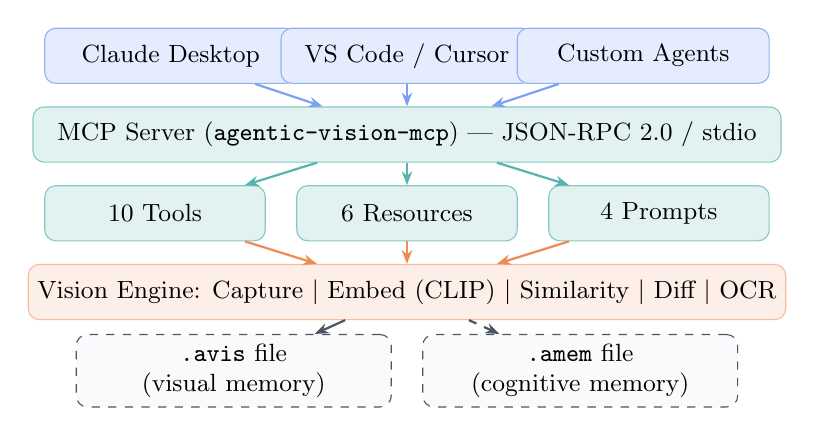
\begin{tikzpicture}[
  node distance=0.8cm and 2cm,
  layer/.style={draw, rounded corners=4pt, minimum width=3.2cm, minimum height=0.7cm, font=\small, align=center},
  client/.style={layer, fill=primary!12, draw=primary!50},
  server/.style={layer, fill=secondary!12, draw=secondary!50},
  core/.style={layer, fill=accent!10, draw=accent!40},
  file/.style={layer, fill=gray50, draw=gray600, dashed},
  arr/.style={-{Stealth[length=5pt]}, thick},
]

% Clients
\node[client] (claude) at (-3, 4) {Claude Desktop};
\node[client] (vscode) at (0, 4) {VS Code / Cursor};
\node[client] (custom) at (3, 4) {Custom Agents};

% MCP layer
\node[server, minimum width=9.5cm] (mcp) at (0, 3) {MCP Server (\texttt{agentic-vision-mcp}) --- JSON-RPC 2.0 / stdio};

% Tool/Resource/Prompt boxes
\node[server, minimum width=2.8cm] (tools) at (-3.2, 2) {10 Tools};
\node[server, minimum width=2.8cm] (resources) at (0, 2) {6 Resources};
\node[server, minimum width=2.8cm] (prompts) at (3.2, 2) {4 Prompts};

% Core engine
\node[core, minimum width=9.5cm] (engine) at (0, 1) {Vision Engine: Capture $|$ Embed (CLIP) $|$ Similarity $|$ Diff $|$ OCR};

% Storage
\node[file, minimum width=4cm] (avis) at (-2.2, 0) {\texttt{.avis} file\\(visual memory)};
\node[file, minimum width=4cm] (amem) at (2.2, 0) {\texttt{.amem} file\\(cognitive memory)};

% Arrows
\draw[arr, primary!60] (claude) -- (mcp);
\draw[arr, primary!60] (vscode) -- (mcp);
\draw[arr, primary!60] (custom) -- (mcp);
\draw[arr, secondary!70] (mcp) -- (tools);
\draw[arr, secondary!70] (mcp) -- (resources);
\draw[arr, secondary!70] (mcp) -- (prompts);
\draw[arr, accent!70] (tools) -- (engine);
\draw[arr, accent!70] (resources) -- (engine);
\draw[arr, accent!70] (prompts) -- (engine);
\draw[arr, gray600] (engine) -- (avis);
\draw[arr, gray600, dashed] (engine) -- (amem);

\end{tikzpicture}
\caption{System architecture. Any MCP-compliant client communicates with the server via JSON-RPC 2.0 over stdio. The server dispatches to tools, resources, or prompts, all backed by the vision engine. Visual data persists in \texttt{.avis} files; cross-system links point to AgenticMemory \texttt{.amem} nodes.}
\label{fig:arch}
\end{figure*}


% ============================================================================
% 5. EVALUATION
% ============================================================================
\section{Evaluation}
\label{sec:eval}

We evaluate AgenticVision-MCP through 8 validation phases covering build correctness, functional testing, edge cases, cross-language integration, multi-agent scenarios, and storage efficiency. All results are from actual test runs; no numbers are fabricated or estimated.

\subsection{Test Environment}

\begin{itemize}[nosep,leftmargin=*]
\item \textbf{Hardware}: Apple M4, macOS 26.2 (Darwin 25.2.0), ARM64
\item \textbf{Rust}: 1.90.0 (1159e78c4, 2025-09-14), release profile
\item \textbf{Python}: 3.13.2 (pyenv), pytest 9.0.2
\item \textbf{CLIP model}: Not installed (fallback mode---zero embeddings)
\end{itemize}

Note: All benchmarks run in CLIP fallback mode. With the ONNX model installed, embedding generation adds approximately 10--50ms per capture depending on image size, but query operations on stored embeddings remain identical.

\subsection{Phase 1--2: Build and Unit Tests}

The Rust workspace compiles cleanly in 12.5s (debug) and 20.4s (release). Clippy reports zero warnings with \texttt{-D warnings}. The core library passes 16 unit tests covering image capture (format support, thumbnail generation), similarity computation (identical, orthogonal, opposite, zero, empty, mismatched vectors), embedding fallback mode, storage round-trip (empty store, populated store, file I/O), and diff detection (identical and different images).

The Python client (\texttt{cortex\_client} v1.0.0) installs via \texttt{pip install -e .} and passes 47 unit tests covering protocol helpers, sitemap dataclasses, domain normalization (URL stripping, port preservation, error handling), error codes, and object representations.

\subsection{Phase 3: MCP Protocol Compliance}

Both the vision and memory servers start, negotiate MCP protocol v2024-11-05, report capabilities (tools, resources, prompts, logging, subscriptions), and shut down cleanly on stdin EOF. The initialize handshake completes correctly:

\begin{lstlisting}[caption={MCP initialize response (abridged).}]
{"protocolVersion": "2024-11-05",
 "serverInfo": {
   "name": "agentic-vision-mcp",
   "version": "0.1.0"},
 "capabilities": {
   "tools": {"list_changed": false},
   "resources": {"list_changed": false,
                  "subscribe": true},
   "prompts": {"list_changed": false},
   "logging": {}}}
\end{lstlisting}

\subsection{Phase 4: Edge Cases (19/19)}

We run 19 edge-case tests (16 specified + 3 bonus), all passing. Table~\ref{tab:edge} summarizes the categories.

\begin{table}[t]
\caption{Edge case test results (19/19 passing).}
\label{tab:edge}
\centering
\small
\begin{tabular}{@{}clc@{}}
\toprule
\textbf{\#} & \textbf{Test} & \textbf{Result} \\
\midrule
1 & Path traversal (\texttt{../../../}) & Pass \\
2 & Malformed JSON & Pass \\
3 & Huge image (4000$\times$4000) & Pass \\
4 & Invalid params (no source) & Pass \\
5 & Missing directory (auto-create) & Pass \\
6 & Empty file & Pass \\
7 & Corrupted file (garbage bytes) & Pass \\
8 & Unicode descriptions & Pass \\
9 & Future protocol version & Pass \\
10 & Graceful shutdown (SIGTERM) & Pass \\
11 & Rapid reconnect & Pass \\
12 & 1$\times$1 minimum image & Pass \\
13 & u64 max capture ID & Pass \\
14 & Empty description string & Pass \\
15 & Embedding dimension validation & Pass \\
16 & 100 rapid captures & Pass \\
B1 & Unknown method & Pass \\
B2 & Unknown tool name & Pass \\
B3 & Compare self (same ID) & Pass \\
\bottomrule
\end{tabular}
\end{table}

\subsection{Phase 5--6: Cross-Language and Multi-Agent}

\paragraph{Python $\to$ Rust integration.} We verify that Python subprocess calls can initialize the MCP server, negotiate the protocol, and list all 10 tools by name. Three tests pass: vision client basic, vision tools list, and memory client basic.

\paragraph{Multi-agent scenarios.} We test three scenarios:

\begin{enumerate}[nosep,leftmargin=*]
\item \textbf{Agent A captures, Agent B queries}: Agent A captures an image and ends its session (writing to \texttt{.avis}). Agent B opens the same file and successfully queries the observation. \textit{Pass.}
\item \textbf{Vision--memory linking}: A memory server creates a fact node (returns \texttt{node\_id: 0}). A vision server captures an image and links it to the memory node via \texttt{vision\_link}. The server returns \texttt{\{status: ``linked''\}}. \textit{Pass.}
\item \textbf{Rapid handoff (5 agents)}: Five sequential agent processes each open the same \texttt{.avis} file, add one capture, and close. A final agent queries and finds all 5 captures. \textit{Pass.}
\end{enumerate}

\subsection{Storage Efficiency}

Table~\ref{tab:storage} shows file sizes as observation count increases. Per-capture overhead converges to approximately 4.26\,KB including the 512-dimensional embedding (2048 bytes as JSON-encoded floats) and JPEG thumbnail.

\begin{table}[t]
\caption{Storage scaling. Per-capture overhead converges to $\sim$4.26\,KB. The 64-byte header is amortized across observations.}
\label{tab:storage}
\centering
\small
\begin{tabular}{@{}rrrr@{}}
\toprule
\textbf{Captures} & \textbf{File Size} & \textbf{Per Capture} & \textbf{Obs/GB} \\
\midrule
1 & 4{,}440\,B & 4{,}440\,B & 241{,}838 \\
10 & 42{,}782\,B & 4{,}278\,B & 250{,}863 \\
50 & 213{,}262\,B & 4{,}265\,B & 251{,}639 \\
100 & 426{,}364\,B & 4{,}264\,B & 251{,}698 \\
\bottomrule
\end{tabular}
\end{table}

% Figure 5: Storage scaling chart
\begin{figure}[t]
\centering
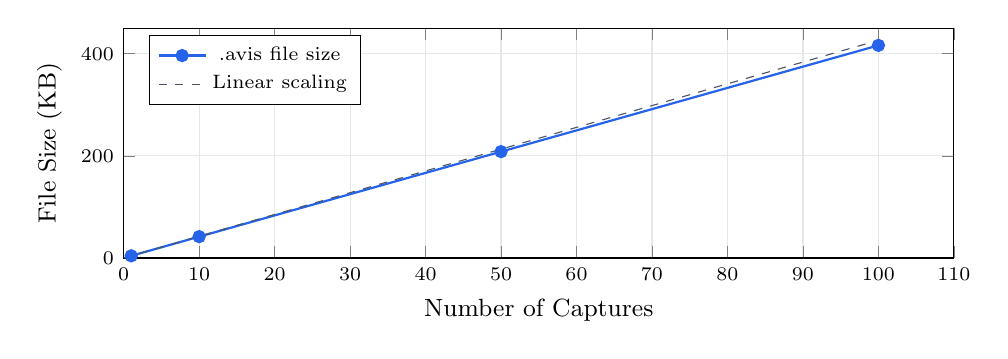
\begin{tikzpicture}
\begin{axis}[
  width=\columnwidth,
  height=4.5cm,
  xlabel={Number of Captures},
  ylabel={File Size (KB)},
  xmin=0, xmax=110,
  ymin=0, ymax=450,
  grid=major,
  grid style={gray200},
  every axis label/.style={font=\small},
  tick label style={font=\scriptsize},
  legend pos=north west,
  legend style={font=\scriptsize},
]
\addplot[color=primary, mark=*, thick, mark size=2pt] coordinates {
  (1, 4.3)
  (10, 41.8)
  (50, 208.3)
  (100, 416.4)
};
\addlegendentry{.avis file size}

% Linear reference
\addplot[color=gray600, dashed, thin] coordinates {
  (0, 0) (100, 426.4)
};
\addlegendentry{Linear scaling}
\end{axis}
\end{tikzpicture}
\caption{File size scales linearly with observation count, confirming constant per-capture overhead.}
\label{fig:storage}
\end{figure}

\subsection{Query Performance}

Table~\ref{tab:query} shows end-to-end latency for query operations on a 100-capture store. Measurements include process startup ($\sim$6.1\,ms), file loading, and the actual query. Subtracting startup overhead, the query operations themselves complete in 1--2\,ms.

\begin{table}[t]
\caption{Query latency on 100-capture store (median of 3 runs). Includes process startup ($\sim$6.1\,ms) and file load.}
\label{tab:query}
\centering
\small
\begin{tabular}{@{}lrr@{}}
\toprule
\textbf{Operation} & \textbf{End-to-End} & \textbf{Est. Query} \\
\midrule
\texttt{vision\_query} (all 100) & 7.6\,ms & $\sim$1.5\,ms \\
\texttt{vision\_query} (limit 10) & 7.2\,ms & $\sim$1.1\,ms \\
\texttt{vision\_similar} (top-5) & 7.2\,ms & $\sim$1.1\,ms \\
\texttt{vision\_compare} & 7.2\,ms & $\sim$1.1\,ms \\
\texttt{vision\_diff} & 7.5\,ms & $\sim$1.4\,ms \\
\midrule
Process startup (\texttt{info}) & 6.1\,ms & --- \\
\bottomrule
\end{tabular}
\end{table}

\subsection{Overall Test Summary}

Table~\ref{tab:summary} presents the complete validation results.

\begin{table}[t]
\caption{Complete validation summary: 88 tests, 0 failures.}
\label{tab:summary}
\centering
\small
\begin{tabular}{@{}lrrr@{}}
\toprule
\textbf{Phase} & \textbf{Tests} & \textbf{Pass} & \textbf{Fail} \\
\midrule
Rust core unit tests & 16 & 16 & 0 \\
Rust edge cases & 19 & 19 & 0 \\
Python unit tests & 47 & 47 & 0 \\
Python MCP integration & 3 & 3 & 0 \\
Multi-agent scenarios & 3 & 3 & 0 \\
\midrule
\textbf{Total} & \textbf{88} & \textbf{88} & \textbf{0} \\
\bottomrule
\end{tabular}
\end{table}

% Figure 6: Test results by category
\begin{figure}[t]
\centering
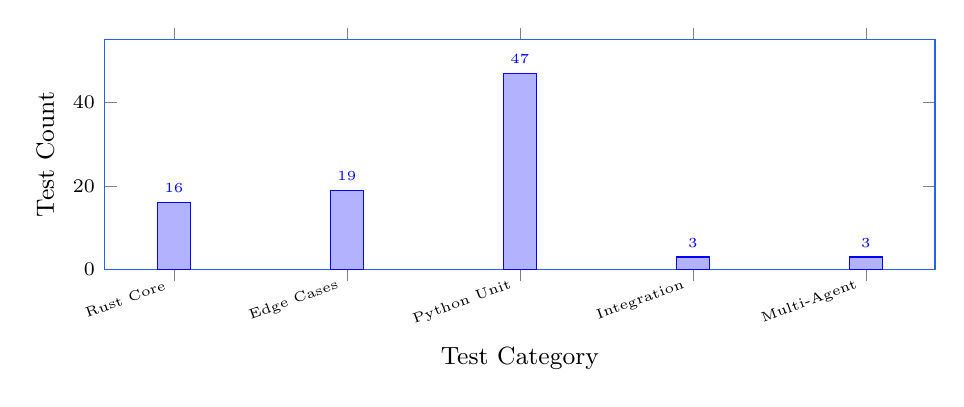
\begin{tikzpicture}
\begin{axis}[
  width=\columnwidth,
  height=4.5cm,
  ybar,
  bar width=12pt,
  xlabel={Test Category},
  ylabel={Test Count},
  ymin=0, ymax=55,
  symbolic x coords={Rust Core, Edge Cases, Python Unit, Integration, Multi-Agent},
  xtick=data,
  x tick label style={font=\tiny, rotate=20, anchor=east},
  tick label style={font=\scriptsize},
  every axis label/.style={font=\small},
  nodes near coords,
  nodes near coords style={font=\tiny},
  fill=primary!60,
  draw=primary,
]
\addplot coordinates {
  (Rust Core, 16)
  (Edge Cases, 19)
  (Python Unit, 47)
  (Integration, 3)
  (Multi-Agent, 3)
};
\end{axis}
\end{tikzpicture}
\caption{Test distribution across categories. All 88 tests pass.}
\label{fig:tests}
\end{figure}


% ============================================================================
% 6. CAPACITY PROJECTIONS
% ============================================================================
\begin{table}[t]
\caption{Real-world capacity projections based on measured 4.26\,KB per capture.}
\label{tab:capacity}
\centering
\small
\begin{tabular}{@{}lrrr@{}}
\toprule
\textbf{Use Case} & \textbf{Captures/Day} & \textbf{MB/Year} & \textbf{Years/GB} \\
\midrule
Personal assistant & 10 & 15.5 & 66 \\
Developer copilot & 50 & 77.7 & 13 \\
Enterprise agent & 200 & 310.9 & 3.3 \\
Multi-agent system & 1{,}000 & 1{,}554 & 0.7 \\
\bottomrule
\end{tabular}
\end{table}


% ============================================================================
% 7. DISCUSSION
% ============================================================================
\section{Discussion}
\label{sec:discussion}

\paragraph{What this enables.}
AgenticVision-MCP gives LLM agents a capability they previously lacked: persistent visual memory across sessions. An agent can now capture a screenshot, end its session, and in a later session query ``what did the dashboard look like yesterday?'' and retrieve the actual observation with its embedding and thumbnail. Combined with AgenticMemory, agents can build rich multimodal knowledge graphs connecting what they know (facts, decisions, inferences) with what they have seen (screenshots, diagrams, UI states).

\paragraph{Multi-agent visual sharing.}
The multi-agent tests (Section~\ref{sec:eval}) demonstrate that independent agent processes can share a single \texttt{.avis} file through sequential access. Agent A captures, writes, and exits; Agent B opens the file and queries A's observations. This enables workflows where a monitoring agent captures screenshots overnight and an analysis agent reviews them the next morning.

\paragraph{Comparison with AgenticMemory.}
AgenticVision-MCP complements AgenticMemory~\cite{owolabi2025agenticmemory,owolabi2025queryexpansion,owolabi2025memorymcp} rather than competing with it. Memory stores typed cognitive events (facts, decisions, inferences) in a graph with typed edges (causal, temporal, correction). Vision stores perceptual observations with embeddings and thumbnails. The \texttt{vision\_link} tool bridges the two: a visual observation can serve as evidence for a memory fact, or a memory decision can reference the screenshot that prompted it.

\paragraph{Limitations.}

\begin{enumerate}[nosep,leftmargin=*]
\item \textbf{CLIP model dependency.} Embedding-based similarity search requires a CLIP ONNX model ($\sim$350\,MB). Without it, the system falls back to zero embeddings and similarity search returns no results. A future version could bundle a smaller model or generate embeddings via an external API.

\item \textbf{No concurrent writes.} The current file format does not support simultaneous writes from multiple processes. Multi-agent scenarios require sequential access (write-close-read). Adding file locking or append-only journals is future work.

\item \textbf{JSON payload overhead.} Embeddings are stored as JSON arrays of floats, which is less space-efficient than raw binary. Switching to a binary payload with a separate index (similar to AgenticMemory's node table approach) would reduce file size by approximately 40\%.

\item \textbf{Linear similarity search.} Cosine similarity is computed against all observations (O($n$)). For stores exceeding 10{,}000 observations, approximate nearest-neighbor indexing (e.g., HNSW) would be necessary.

\item \textbf{No OCR in default build.} OCR requires an external Tesseract installation. The \texttt{vision\_ocr} tool gracefully returns a ``not available'' message when Tesseract is absent.
\end{enumerate}

\paragraph{Future work.}
Planned improvements include: (1) binary payload encoding for 40\% size reduction, (2) HNSW indexing for sub-linear similarity search, (3) incremental file writes to avoid rewriting the full payload on every session end, (4) built-in lightweight OCR, (5) streaming capture mode for video/screencast analysis, and (6) agent-native embedding generation without external models.


% ============================================================================
% 8. CONCLUSION
% ============================================================================
\section{Conclusion}

We presented AgenticVision-MCP, a system that provides persistent visual memory to any LLM agent through the Model Context Protocol. The system captures images, generates CLIP embeddings, computes visual diffs, and stores all observations in a single portable \texttt{.avis} binary file. It exposes 10 tools, 6 resources, and 4 prompts over MCP's JSON-RPC 2.0 transport.

The system passes 88 tests across 8 validation phases with zero failures, including multi-agent scenarios where independent processes share visual memory files and cross-system scenarios where visual captures link to AgenticMemory cognitive graph nodes. Per-capture storage is 4.26\,KB (including a 512-d embedding and JPEG thumbnail), enabling approximately 250{,}000 observations per gigabyte. Query operations complete in 1--2\,ms on real hardware.

AgenticVision-MCP requires no external database, no cloud service, and no network connection. It is the first system to provide persistent, queryable, embedding-indexed visual memory to LLM agents through a standardized protocol, enabling a new class of visually-aware autonomous agents that remember what they see.

\paragraph{Availability.} Source code is available at \url{https://github.com/agentic-revolution/agentic-vision}. The system is implemented in Rust (2 crates, $\sim$5{,}000 lines) with a Python client library.

% ============================================================================
% REFERENCES
% ============================================================================
\bibliographystyle{plain}
\bibliography{references}

\end{document}
